
\begin{table*}[t]
\centering
\footnotesize
\setlength{\tabcolsep}{2.3pt}
\renewcommand{\arraystretch}{1.08}
\newcommand{\benchref}[2]{\parbox[t]{3.35cm}{#1\\[-1pt]{\scriptsize #2}}}
\begin{tabular}{@{}p{3.35cm}c c c*{7}{c}@{}}
\toprule
Benchmark & \shortstack{Decision\\maker} & \shortstack{Data\\grounded} & Horizon & \shortstack{Price--\\Inv.} & \shortstack{Perish./\\Stockout} & Shelf & Reviews & Supplier & News & Finance \\
\midrule
\benchref{RetailSynth}{\citep{xia2023retailsynth}} & Policy & \xmark & Medium & \cmark & \xmark & \xmark & \xmark & \xmark & \xmark & \xmark \\
\benchref{Promo-RL}{\citep{xia2024simulationretailpromotions}} & Policy & \xmark & Medium & \cmark & \xmark & \xmark & \xmark & \xmark & \xmark & \xmark \\
\benchref{FreshRetailNet}{\citep{wang2025freshretailnet}} & None & \cmark & Static & \xmark & \cmark & \xmark & \xmark & \xmark & \xmark & \xmark \\
\benchref{Transaction sim.}{\citep{tkachuk2024consumertransactions}} & None & \cmark & Static & \xmark & \cmark & \xmark & \xmark & \xmark & \xmark & \xmark \\
\benchref{ShoppingBench}{\citep{wang2025shoppingbench}} & Agents & \cmark & Medium & \xmark & \xmark & \xmark & \cmark & \xmark & \xmark & \xmark \\
\benchref{WebShop}{\citep{3webshopscalablerealworldweb}} & Agents & \cmark & Medium & \xmark & \xmark & \xmark & \cmark & \xmark & \xmark & \xmark \\
\benchref{OFCOURSE}{\citep{OFCOURSE}} & Policy & \xmark & Long & \xmark & \cmark & \xmark & \xmark & \xmark & \xmark & \xmark \\
\benchref{Inventory opt.}{\citep{inventory}} & Policy & \xmark & Long & \xmark & \cmark & \xmark & \xmark & \xmark & \xmark & \xmark \\
\benchref{MARLIM}{\citep{leluc2023marlimmultiagentreinforcementlearning}} & Policy & \xmark & Long & \xmark & \cmark & \xmark & \xmark & \xmark & \xmark & \xmark \\
\benchref{InvAgent}{\citep{invagentlargelanguagemodel}} & Agents & \xmark & Medium & \xmark & \cmark & \xmark & \xmark & \xmark & \xmark & \xmark \\
\benchref{AIM-Bench}{\citep{aimbenchevaluatingdecisionmakingbiases}} & Agents & \xmark & Medium & \xmark & \cmark & \xmark & \xmark & \xmark & \xmark & \xmark \\
\benchref{VendingBench}{\citep{backlund2025vendingbenchbenchmarklongtermcoherence,andonlabs2025vendingbench2}} & Agents & \xmark & Long & \cmark & \xmark & \xmark & \xmark & \cmark & \xmark & \cmark \\
\textbf{RetailBench} & \textbf{Agents} & \cmark & \textbf{Long} & \cmark & \cmark & \cmark & \cmark & \cmark & \cmark & \cmark \\
\bottomrule
\end{tabular}
\caption{Comparison with related retail, supply-chain, e-commerce, and long-horizon agent benchmarks. The table emphasizes the decision surface exposed to the decision maker. ``Agents'' denotes LLM/tool-using agents, ``Policy'' denotes learned optimization or RL policies, and ``None'' denotes datasets or simulators without an autonomous decision maker. A checkmark indicates that the corresponding axis is explicitly modeled as an environment state, action, or evaluation target.}
\label{tab:benchmark_axes}
\end{table*}

\subsection{Simulator Modules}
\label{app:simulator_modules}

RetailBench follows the seven-module organization shown in Figure~\ref{fig:retailbench_environment}: Inventory, Suppliers \& Orders, Shelf, Customer Demand, Reviews \& Returns, News Events, and Finance \& Records. Static product attributes, including identity, category, shelf life, retail price, historical sales summaries, and review summaries, are shared across these modules. The modules are coupled through the daily transition process: orders create delayed deliveries, shelf-assortment decisions determine customer-facing availability, demand is realized as sales, reviews and returns update feedback signals, news changes demand or supply conditions, and finance records cash-flow outcomes and store viability.

\paragraph{Inventory.}
The inventory module tracks physical stock state, including on-hand units, item age, sellable quantity, capacity constraints, stockouts, expirations, and waiting items that cannot yet enter inventory because of capacity limits. It determines the feasibility constraints for procurement, shelving, and sales.

\paragraph{Shelf.}
The shelf module enforces shelf-capacity constraints and determines the customer-facing assortment. At each day $t$, it maintains an active assortment $V_t \subseteq \mathcal{J}$ subject to the capacity constraint $|V_t| \le C^{\mathrm{shelf}}$. Stocked products outside $V_t$ remain in inventory but are not visible to customers and therefore cannot generate demand.

\paragraph{Suppliers \& Orders.}
The suppliers-and-orders module provides five procurement candidates per product, each with cost, quality, and delivery-time profiles. Costs are grounded in Dominick's, and quality tiers follow documented price--quality relationships in private-label retailing~\citep{supplychain}; supplier choices affect procurement expenditure, delivery timing, return risk, reviews, and future inventory availability. Replenishment orders are converted into delayed deliveries that enter inventory on later days when capacity allows.

\paragraph{Customer Demand.}
Following RetailSynth~\citep{xia2023retailsynth}, customer choice follows an MNL model~\citep{mcfadden_conditional_1974}. Daily traffic comes from Dominick's~\citep{DominicksDataset}. The simulator first samples category demand from power-aggregated shelf-visible attraction~\citep{nakanishi1974mci}, then allocates it across visible products. The corresponding update equations are given in Appendix~\ref{app:simulator_update_equations}.

\paragraph{Reviews \& Returns.}
The reviews-and-returns module converts realized sales and supplier quality into post-sale feedback. Sold items can generate product-level reviews, which update rating summaries and later demand through $\rho^{\mathrm{rev}}_{jt}$. Returned units are sampled from supplier-quality-dependent return probabilities, logged at the product and supplier level, and deducted from realized revenue. Thus, supplier quality affects both customer feedback and return pressure.

\paragraph{News Events.}
The news-events module samples observable news text with hidden simulator metadata specifying impact scope, target category or product, direction, strength, affected side, and duration. Demand-side news changes product attraction through $\rho^{\mathrm{news}}_{jt}$, while supply-side news changes supplier costs through $\delta^{\mathrm{sup}}_{jt}$.

\paragraph{Finance \& Records.}
The finance-and-records module tracks revenue, procurement cost, returns, rent, cash, inventory value, pending-order value, net worth, and persistent sales, supplier, review, return, and news records. At each day transition, the simulator applies deliveries, shelf-constrained demand realization, sales, feedback updates, expiration, rent, cash-flow updates, and next-day supplier/news changes.

\subsection{State and Action Spaces}
\label{app:state_action_spaces}

We construct the environment using real-world retail data from the Dominick’s dataset \citep{DominicksDataset}. From the 20 available product categories, we select 96 products with the most complete and informative sales records. The richness of these observations enables reliable modeling of the relationship between pricing decisions and realized demand.

\paragraph{Key Symbols.}
Let $\mathcal{J}$ denote the set of selected products, with cardinality $|\mathcal{J}| = J$ (where $J=96$ in our experiments). Each product $j \in \mathcal{J}$ belongs to a product category $\mathrm{cat}(j) \in \{1,\ldots,20\}$. For each product $j$, let $\mathcal{K}(j)$ denote its associated supplier set, with $|\mathcal{K}(j)| = 5$. Let $V_t\subseteq\mathcal{J}$ denote the product set placed on shelf on day $t$.

\paragraph{State and action spaces.}
The simulator state space is $\mathcal{S}=\mathcal{S}^{\mathrm{prod}}\times\mathcal{S}^{\mathrm{inv}}\times\mathcal{S}^{\mathrm{shelf}}\times\mathcal{S}^{\mathrm{sup}}\times\mathcal{S}^{\mathrm{dem}}\times\mathcal{S}^{\mathrm{ext}}\times\mathcal{S}^{\mathrm{fin}}$, covering product attributes and prices, inventory and pending deliveries, shelf assortment, supplier candidates, demand signals, external news, and financial accounting. The action space is $\mathcal{A}=\mathcal{A}^{\mathrm{read}}\cup\mathcal{A}^{\mathrm{other}}\cup\mathcal{A}^{\mathrm{act}}$: $\mathcal{A}^{\mathrm{read}}$ contains observation tools for funds, inventory, shelf status, product prices, costs, sales/profit history, supplier quotes, notes, review-rating summaries, supplier-return-rate summaries, and news; $\mathcal{A}^{\mathrm{other}}$ contains constrained analysis tools such as \texttt{execute\_code}; and $\mathcal{A}^{\mathrm{act}}$ contains \texttt{place\_order}, \texttt{modify\_product\_price}, \texttt{set\_shelf\_products}, \texttt{add\_note}, \texttt{remove\_note}, and \texttt{end\_today}.

\subsubsection{Product State \texorpdfstring{$S_t^{\text{prod}}$}{S t prod}}

For each product $j$, we maintain a set of static attributes together with time-varying operational signals:
\begin{equation}
S_{t,j}^{\text{prod}} =
\big(
\texttt{id}_j,\ \texttt{desc}_j,\ L_j,\ p_{jt},\ \mathbf{h}^{\text{sales}}_{j,t},\ \mathbf{r}_{j,t}
\big).
\end{equation}
Here, $\texttt{id}_j$ and $\texttt{desc}_j$ denote the unique identifier and textual description of product $j$, respectively. $L_j$ denotes the shelf life (in days), and $p_{jt}$ is the retail price on day $t$. The term $\mathbf{h}^{\text{sales}}_{j,t}$ encodes historical sales statistics, while $\mathbf{r}_{j,t}$ summarizes aggregated customer review signals, such as average rating and review volume.

\paragraph{Data grounding.}
The product set and cost priors are constructed from the Dominick’s dataset \citep{DominicksDataset}. Historical sales records from the same source are used to calibrate the demand model.

\subsubsection{Inventory State \texorpdfstring{$S_t^{\text{inv}}$}{S t inv}}

Inventory is represented at the product level with age tracking. Let $I_{jt}$ denote the on-hand units of product $j$ at the beginning of day $t$. To support shelf-life constraints and depreciation, we track the arrival time and remaining shelf life of each unit.

\paragraph{Capacity constraint and pending queue.}
Let $\mathrm{Cap}$ denote the total inventory capacity of the store. If incoming replenishment orders would violate this constraint, excess units are placed into a first-in-first-out (FIFO) pending queue $\mathcal{Q}_t$ and become available only after sufficient inventory space is released:
\begin{equation}
\sum_{j\in\mathcal{J}} \sum_{a=0}^{L_j} I_{jt}^{(a)} \le \mathrm{Cap}.
\end{equation}

\paragraph{Stockout signal.}
When realized demand exceeds the available sellable inventory of product $j$ on day $t$, a stockout indicator is triggered. This signal is recorded at the end of day $t$ and exposed to the agent as explicit operational feedback.

\paragraph{Expiration and destruction.}
At each day transition, inventory units whose residence time exceeds their shelf life are removed from the system.

\paragraph{Shelf assortment.}
RetailBench additionally tracks an active shelf assortment $V_t$. The shelf has finite product capacity:
\begin{equation}
V_t \subseteq \mathcal{J}, \qquad |V_t| \le C^{\mathrm{shelf}}.
\end{equation}
Only products in $V_t$ are visible to customer demand; newly delivered inventory remains off shelf until the agent updates $V_t$ through the shelf-assortment action.

\subsubsection{Supply Chain State \texorpdfstring{$S_t^{\text{sup}}$}{S t sup}}

Each product $j$ is associated with a set of suppliers $k \in \mathcal{K}(j)$. The supplier state includes procurement price $c_{jk}$, quality level $q_{jk}$, and delivery-time distribution:
\begin{equation}
S_{t,j}^{\text{sup}} =
\big\{(c_{jk}, q_{jk}, \mathcal{L}_{jk}) : k \in \mathcal{K}(j)\big\}.
\end{equation}
Delivery time $\ell_{jk} \sim \mathcal{L}_{jk}$ is sampled when an order is placed. Procurement prices are discretized into tiers using Dominick’s cost signals \citep{DominicksDataset}, following empirically observed positive correlations between price tier and quality level \citep{supplychain}.

\paragraph{Enforced diversity.}
To avoid degenerate supplier configurations, we enforce that each product has (i) one supplier with maximal quality, (ii) one supplier with minimal price and minimal quality, and remaining suppliers spanning intermediate price–quality levels.

\subsubsection{Demand Signals and Demand Generation}
\label{app:demand}

Demand-related components capture customer traffic, shelf-visible choice sets, and stochastic sales generation. We define
\begin{equation}
S_t^{\text{dem}} =
\big(
N_t,\ \{A^0_{jt}\}_{j\in\mathcal{J}},\
\{\rho^{\mathrm{rev}}_{jt}\}_{j\in\mathcal{J}},\
\{\rho^{\mathrm{news}}_{jt}\}_{j\in\mathcal{J}}
\big),
\end{equation}
where $N_t$ denotes daily customer traffic, $A^0_{jt}$ is the calibrated base attraction, and $\rho^{\mathrm{rev}}_{jt}$ and $\rho^{\mathrm{news}}_{jt}$ are bounded demand-side effects from reviews and news.

\paragraph{Customer traffic.}
Daily customer traffic is derived from the Dominick’s dataset~\citep{DominicksDataset}.

\paragraph{Consumer choice and demand generation.}
Given traffic $N_t$, prices $\{p_{jt}\}_{j\in\mathcal{J}}$, shelf assortment $V_t$, review signals, and active news, RetailBench uses the attraction model in Equations~\ref{eq:base_attraction}--\ref{eq:demand_sales}. The current implementation aggregates shelf-visible product attractions within each category using a power mean, samples category-level demand against an outside option, allocates category demand with a multinomial draw over relative product attractions, and caps realized sales by sellable inventory. If $j\notin V_t$, then product $j$ cannot receive demand on that day.

\subsubsection{External Information \texorpdfstring{$S_t^{\text{ext}}$}{S t ext} (News Module)}

We maintain a set of active news events $\mathcal{E}_t$. Each event $e \in \mathcal{E}_t$ is represented as
\begin{equation}
\begin{aligned}
e = (&\texttt{type},\ \texttt{scope},\ \texttt{target},\\
     &\texttt{side},\ \texttt{sign},\ \eta,\\
     &\texttt{text},\ \texttt{ttl})
\end{aligned}
\end{equation}

where \texttt{scope} $\in \{\text{macro}, \text{category}, \text{product}, \text{neutral}\}$,
\texttt{side} $\in \{\text{demand}, \text{supply}, \text{both}\}$,
\texttt{sign} $\in \{+1,-1\}$,
$\eta$ denotes impact magnitude, and \texttt{ttl} is the time-to-live in days. News texts are grounded in financial-news-articles~\citep{ashraq2025financialNewsArticles} and expanded into retail-relevant events through LLM-assisted rewriting and metadata annotation.

\paragraph{Impact application.}
News impacts are incorporated into (i) demand utilities and/or (ii) supplier prices depending on \texttt{side} and \texttt{scope}. Neutral news has $\eta = 0$ by design.

\subsubsection{Simulator Update Equations}
\label{app:simulator_update_equations}

This section gives the detailed equations summarized in Section~\ref{sec:module_logic}.

\paragraph{Supply price update.}
Let $\bar c_{jkt}$ be the base procurement price for supplier $k$ and product $j$ on day $t$, and let $\delta^{\mathrm{sup}}_{jt}$ be the active supply-side news effect matched to product $j$, its category, or the macro scope. The daily procurement price exposed to the agent is
\begin{equation}
c_{jkt}=\bar c_{jkt}\bigl(1-\delta^{\mathrm{sup}}_{jt}\bigr).
\label{eq:supply_price}
\end{equation}
Positive supply news lowers procurement cost, while negative supply news raises it.

\paragraph{Attraction and sales.}
The base product attraction combines historical preference, seasonality, price sensitivity, and stochastic demand noise:
\begin{equation}
\begin{aligned}
A^{0}_{jt}
=\exp\!\Big(&\alpha_j+
\bigl(\beta_j+\beta^s_j\sin(2\pi w_t/52)\\
&+\beta^c_j\cos(2\pi w_t/52)\bigr)p_{jt}
+\epsilon_{jt}\Big).
\end{aligned}
\label{eq:base_attraction}
\end{equation}
Reviews and news multiplicatively adjust this attraction:
\begin{equation}
A_{jt}=A^{0}_{jt}\bigl(1+\rho^{\mathrm{rev}}_{jt}+\rho^{\mathrm{news}}_{jt}\bigr).
\label{eq:adjusted_attraction}
\end{equation}
Let $V_{ct}=\{j\in V_t:\mathrm{cat}(j)=c\}$ be the shelf-visible product set in category $c$. Given daily traffic $N_t$, RetailBench samples category-level purchase volume and allocates it by relative attraction among shelf-visible products:
\begin{equation}
\begin{aligned}
G_{ct}
&=\left(\sum_{j\in V_{ct}} A_{jt}^{\rho}\right)^{1/\rho},\\
\tilde Y_{ct}
&\sim \mathrm{Binomial}\!\left(N_t,\frac{G_{ct}}{1+G_{ct}}\right),\\
\pi_{jt|c}
&=\frac{A_{jt}}{\sum_{i\in V_{ct}}A_{it}}, \quad j\in V_{ct},\\
\hat{\mathbf{y}}_{ct}
&\sim \mathrm{Multinomial}\!\left(\tilde Y_{ct},\boldsymbol{\pi}_{ct}\right),\\
y_{jt}
&=\min\!\left(\hat y_{jt}, I_{jt}^{\mathrm{sellable}}\right).
\end{aligned}
\label{eq:demand_sales}
\end{equation}

\paragraph{Review effect.}
Review text is grounded in Amazon Reviews 2023~\citep{hou2024bridging}. During simulation, sold units can generate reviews; the rating is sampled from supplier quality and the text is sampled from the matching category--rating--dimension pool. The demand effect is computed from the difference between recent and initial rating:
\begin{equation}
\rho^{\mathrm{rev}}_{jt}
=g_{\mathrm{cat}(j)}(\bar r_{jt})-g_{\mathrm{cat}(j)}(r^{0}_{j}),
\label{eq:review_effect}
\end{equation}
where $g_{\mathrm{cat}(j)}(\cdot)$ is a category-specific smooth rating-gain function, $\bar r_{jt}$ is the recent average rating, and $r^{0}_{j}$ is the initial rating.

\paragraph{News effect.}
Each news event is stored as
\begin{equation}
e=(m,\tau,\texttt{side},\texttt{direction},s,\texttt{text},\texttt{ttl}),
\label{eq:news_record}
\end{equation}
where $m$ is event mode, $\tau$ is target scope, \texttt{side} specifies demand, supply, or both, $s$ is impact strength, and \texttt{ttl} controls how long the event remains active. Demand-side news contributes
\begin{equation}
\rho^{\mathrm{news}}_{jt}
=\lambda\sum_{e\in\mathcal{E}_t:\,e\sim j}
w_{m(e)}\,\mathrm{sgn}(e)\,s_e,
\label{eq:news_effect}
\end{equation}
where $e\sim j$ indicates that the event matches the product, its category, or the macro scope; $w_{m(e)}$ is the mode weight; and $\lambda$ is the global impact scale. Supply-side events analogously define $\delta^{\mathrm{sup}}_{jt}$ in Equation~\ref{eq:supply_price}.

\subsubsection{Financial State \texorpdfstring{$S_t^{\text{fin}}$}{S t fin}}

Let $F_t$ denote available funds at the start of day $t$. Net worth is computed as
\begin{equation}
\mathrm{NW}_t = F_t + \sum_{j\in\mathcal{J}} \sum_{a=0}^{L_j} I_{jt}^{(a)} \cdot v_j(a),
\end{equation}
where $v_j(a)$ denotes the per-unit value at age $a$. We adopt linear shelf-life depreciation:
\begin{equation}
v_j(a) = c_j \cdot \max\!\left(0,\ 1 - \frac{a}{L_j}\right),
\end{equation}
with $c_j$ denoting a reference procurement cost (e.g., the mean or realized supplier cost).

\subsubsection{Action Space Details}
\label{app:action_space_details}

RetailBench exposes actions through typed tools. Read-only tools instantiate $\Omega$ and do not modify simulator state; other tools provide constrained analysis over observations; state-changing tools instantiate $T$.

\paragraph{Read-only tools.}
\begin{itemize}[leftmargin=*,nosep]
    \item \texttt{view\_funds\_and\_date}: returns current funds, date, and rent context.
    \item \texttt{view\_inventory}: reports on-hand units, waiting-capacity items, incoming quantities, and open supplier orders.
    \item \texttt{view\_shelf\_status}: reports active shelf assortment, shelf capacity, and on-shelf product summaries.
    \item \texttt{view\_product\_prices}: returns current selling prices for selected products.
    \item \texttt{view\_product\_inventory\_cost}: summarizes average procurement cost and inventory age.
    \item \texttt{view\_sales\_profit\_history}: returns historical sales, average selling price, and realized profit.
    \item \texttt{view\_current\_date\_supplier\_prices}: returns current supplier quotes.
    \item \texttt{view\_supplier\_price\_history}: returns historical supplier prices for a product.
    \item \texttt{view\_notes}: returns the agent's stored cross-day notes.
\end{itemize}

\paragraph{Conditional observation tools.}
\begin{itemize}[leftmargin=*,nosep]
    \item \texttt{view\_product\_avg\_ratings}: exposes product-level average ratings when review feedback is enabled.
    \item \texttt{view\_supplier\_returns\_avg\_rate}: exposes supplier-level return rates, optionally restricted to selected products.
    \item \texttt{view\_today\_news}: lists current news IDs and titles when news is enabled.
    \item \texttt{view\_news\_detail}: returns the observable content of a selected news item.
    \item \texttt{view\_news\_history}: returns news records over a date range.
\end{itemize}

\paragraph{Other/analysis tools.}
\begin{itemize}[leftmargin=*,nosep]
    \item \texttt{execute\_code}: runs constrained Python for read-only analysis over observations. It can compute summaries, rank products, and compare suppliers, but mutation tools are unavailable inside the sandbox.
\end{itemize}

\paragraph{State-changing tools.}
\begin{itemize}[leftmargin=*,nosep]
    \item \texttt{place\_order}: places a multi-product order through a selected supplier, deducts procurement cost, samples delivery time, and schedules future inventory arrivals.
    \item \texttt{modify\_product\_price}: updates the retail price $p_{jt}$ of product $j$.
    \item \texttt{set\_shelf\_products}: replaces the active shelf assortment subject to $|V'|\le C^{\mathrm{shelf}}$.
    \item \texttt{add\_note} and \texttt{remove\_note}: update cross-day notes.
    \item \texttt{end\_today}: applies $T_{\mathrm{day}}$ over deliveries, shelf-visible demand, sales, reviews, returns, expiration, rent, cash-flow updates, and next-day supplier/news changes.
\end{itemize}

\subsection{Environment Setting}
\label{appendix:env_setting}

RetailBench provides a single released environment configuration for all reported evaluations.

\begin{itemize}
    \item \textbf{Time Range:}
    \begin{itemize}
        \item Data begin time: 06/06/91
        \item Data end time: 12/31/95
        \item Store begin time: 09/07/91
        \item Store ID: 15
    \end{itemize}
    
    \item \textbf{Financial Parameters:}
    \begin{itemize}
        \item Initial funds: 30,000
        \item Daily rent: 600
        \item Inventory capacity: 15,000
        \item Shelf capacity: 40 products
    \end{itemize}
    
    \item \textbf{Feature Enablement:}
    \begin{itemize}
        \item Review enabled: \texttt{True}
        \item Review ratio: 0.05
        \item News enabled: \texttt{True}
        \item Shelf constraint enabled: \texttt{True}
    \end{itemize}
    
    \item \textbf{News Configuration:}
    \begin{itemize}
        \item News impact base scale: 0.4
        \item News daily count: 20
        \item News random seed: 42
        \item News sample ratios:
        \begin{itemize}
            \item Neutral: 0.9
            \item Single category: 0.02
            \item Macro all: 0.03
            \item product level: 0.05
        \end{itemize}
        \item News impact mode weights:
        \begin{itemize}
            \item Neutral: 0.0
            \item Macro all: 1.0
            \item Single category: 1.0
            \item product level: 1.2
        \end{itemize}
    \end{itemize}
    
    \item \textbf{Selected Categories (20 categories):}
    \begin{itemize}
        \item Bathroom\_Tissues, Beer, Bottled\_Juices, Canned\_Soup, Canned\_Tuna
        \item Cereals, Cheeses, Cigarettes, Cookies, Crackers
        \item Dish\_Detergent, Fabric\_Softeners, Front\_end\_candies, Frozen\_Entrees
        \item Frozen\_Juices, Oatmeal, Paper\_Towels, Snack\_Crackers
        \item Soft\_Drinks, Toothpastes
    \end{itemize}
    
    \item \textbf{Category Effects:} All categories have a uniform effect of -0.1
    
    \item \textbf{Random Seed:} 42
\end{itemize}

\subsection{Hand-Crafted Policy}
\label{appendix:handcrafted_policy}

The non-LLM reference policy is a deterministic, quality-based store-operation rule used only as an approximate oracle-style reference. It is not a language-agent baseline: it has direct access to structured simulator fields such as supplier quality scores and news impact values, and it does not face prompt length, tool-selection, memory, or action-formatting constraints. The reported run uses the released environment with $n_{\mathrm{cat}}=2$ products per category, shelf capacity $C^{\mathrm{shelf}}=40$, and replenishment multiplier $B=6$, selected by a parameter sweep over the shelf-constrained setting.

\begin{algorithm}[t]
\small
\caption{Hand-crafted quality-based policy}
\label{alg:handcrafted_policy}
\begin{algorithmic}[1]
\Require Horizon $T$, categories $\mathcal{C}$, products $\mathcal{J}$, shelf capacity $C^{\mathrm{shelf}}$, per-category product count $n_{\mathrm{cat}}$, bulk multiplier $B$.
\State Select $\mathcal{U}\leftarrow\emptyset$.
\For{each category $c\in\mathcal{C}$}
    \State Rank products in $c$ by historical total profit before the store start date.
    \State Add the top $n_{\mathrm{cat}}$ products to $\mathcal{U}$.
\EndFor
\State Set shelf assortment $V_0$ to a category-diverse subset of $\mathcal{U}$ with $|V_0|\le C^{\mathrm{shelf}}$.
\For{day $t=1,\ldots,T$}
    \If{funds are negative for 10 consecutive days}
        \State Terminate the rollout.
    \EndIf
    \State Observe funds, news, inventory, shelf status, recent sales, and supplier quotes.
    \For{each product $j\in\mathcal{U}$}
        \State $I_j \leftarrow$ on-hand units plus waiting-capacity units for product $j$.
        \State Choose supplier $k^\star=\arg\max_k(q_{jk},-c_{jkt})$.
        \State Estimate price $p^\star_j$ by maximizing mean 30-day historical profit:
        \Statex \hspace{\algorithmicindent} $p^\star_j=\arg\max_p \operatorname{mean}\{(p-c_{jk^\star t})\,y_{j\tau}:p_{j\tau}=p\}$.
        \State Let $\hat d_j$ be the mean historical sales at $p^\star_j$; use $\hat d_j=10$ if no record is available.
        \State Compute news multiplier $m_j=\operatorname{clip}((1+\eta^{\mathrm{need}}_j)(1+\eta^{\mathrm{sup}}_j),0.5,2.0)$.
        \State Set target demand $\tilde d_j \leftarrow m_j\hat d_j$.
        \If{$p^\star_j$ exists}
            \State Call \texttt{modify\_product\_price}$(j,p^\star_j)$.
        \EndIf
        \State Let $Q_j$ be the pending order quantity for product $j$.
        \State Let $R_j\leftarrow B\tilde d_j$ and $O_j\leftarrow \max(1,\lfloor B\tilde d_j\rfloor)$.
        \If{$I_j\le R_j$ and $Q_j<O_j$}
            \State $a_j\leftarrow \min(O_j-Q_j,\ \text{available inventory capacity}-100)$.
            \If{$a_j>0$}
                \State Call \texttt{place\_order} for $a_j$ units of product $j$ from supplier $k^\star$.
            \EndIf
        \EndIf
    \EndFor
    \State Call \texttt{end\_today}.
\EndFor
\end{algorithmic}
\end{algorithm}

\subsection{Four-Stage Diagnostic Metrics}
\label{appendix:stage_metrics}

This section defines the stage-level diagnostics used in Section~\ref{sec:failure_pattern_analysis}. The metrics are computed after each rollout by aligning three sources: tool-call traces, simulator records, and realized delayed events. They are diagnostic rather than reward functions. In particular, some quantities use retrospective information or hidden simulator fields to explain agent behavior; they should not be interpreted as information available to the agent at decision time.

We evaluate the daily operational loop in four stages. Stage 1 asks whether important products entered the agent's action set. Stage 2 asks whether the agent gathered the evidence needed before acting. Stage 3 asks whether the gathered evidence was converted into quality-adjusted prices and supplier choices. Stage 4 asks whether the agent later revisited products affected by delayed consequences. Unless otherwise noted, we use a seven-day follow-up window and a three-day lookback window for high-demand coverage.

\paragraph{Stage 1: Product candidate selection.}
This stage measures whether the agent allocates attention to a sufficiently broad and relevant product set. From the tool traces, we extract executed state-changing product actions, including replenishment orders and price updates. Let $\mathcal{U}_{t}$ be the set of products receiving at least one such action on day $t$. Let $\mathcal{H}_{t}$ be the retrospective high-demand set, formed by the top-10 realized-sales products on day $t$ together with products that experienced stockout on that day. We report
\begin{equation}
\mathrm{Acted/day}
=\frac{1}{T}\sum_{t=1}^{T}|\mathcal{U}_{t}|,
\end{equation}
\begin{equation}
\mathrm{HighDemandCov}
=1-\frac{\sum_t|\mathcal{H}_{t}\setminus\mathcal{U}_{t-w:t}|}
{\sum_t|\mathcal{H}_{t}|},
\end{equation}
where $\mathcal{U}_{t-w:t}=\bigcup_{\tau=\max(1,t-w)}^{t}\mathcal{U}_{\tau}$ and $w=3$. \textbf{Acted/day} captures action breadth. \textbf{HighDemandCov} captures whether high-demand or stockout-affected products received recent operational attention. Auxiliary diagnostics include the number of distinct acted products, category coverage, action concentration, the top-10 product action share, and whether an acted product sells within seven days. These auxiliary quantities help distinguish a genuinely broad policy from a narrow policy that repeatedly acts on only a few products.

\paragraph{Stage 2: evidence acquisition.}
This stage measures whether a product action is supported by relevant same-day observations. Let $\mathcal{B}$ denote the evaluated executed product actions. For each action $a\in\mathcal{B}$, we define a required evidence set $\mathcal{R}(a)$. Replenishment orders require inventory, recent sales, supplier prices, and supplier-quality proxies such as customer ratings or supplier return rates. Price updates require current price, cost, inventory, and recent sales/profit history. Let $\mathcal{Q}(a)$ be the evidence categories queried earlier on the same day before $a$, and let $m_a=1$ if at least one required category is missing. We report
\begin{equation}
\mathrm{QDepth}
=\frac{1}{|\mathcal{B}|}\sum_{a\in\mathcal{B}}
\frac{|\mathcal{Q}(a)\cap\mathcal{R}(a)|}{|\mathcal{R}(a)|}.
\end{equation}
\begin{equation}
\mathrm{Completeness}
=1-\frac{1}{|\mathcal{B}|}\sum_{a\in\mathcal{B}}m_a.
\end{equation}
\textbf{QDepth} measures partial evidence coverage, while \textbf{Completeness} requires all action-critical evidence categories to be present. We also record the average gap between the last relevant query and the action, the number of distinct evidence tools used before an action, and same-day query--action overlap. For the hand-crafted policy, \textbf{QDepth} and \textbf{Completeness} are set to 1 because the policy is a structured rule system whose inputs explicitly include the required inventory, demand, supplier, and price fields.

\paragraph{Stage 3: action conversion.}
This stage measures whether evidence is converted into economically meaningful actions. For price actions, let $p_a$ be the selected price and $p_a^\star$ be the historical-profit optimum estimated from visible sales and cost records. We first compute the absolute percentage distance
\begin{equation}
d_a=100\cdot\frac{|p_a-p_a^\star|}{p_a^\star}.
\end{equation}
The text reports the run-level mean distance $\bar d_r$ directly. For the normalized diagnostic plot in Figure~\ref{fig:failure_diagnostics}(b), we convert distance into an upper-right-is-better run-level score:
\begin{equation}
\mathrm{PriceClose}_r=1-\frac{\bar d_r}{\max_{r'}\bar d_{r'}},
\end{equation}
where the maximum is taken over valid plotted runs. Thus larger values indicate prices closer to the historical-profit optimum.

For supplier actions, let $r_a^{q}$ be the rank of the chosen supplier by raw quality among $K(a)$ same-product candidates, where rank 1 is best. We report
\begin{equation}
\mathrm{SupplierQual}(a)=
\frac{K(a)-r_a^{q}}{K(a)-1}.
\end{equation}
Because each product has five suppliers in our environment, this score maps the best-quality supplier to 1 and the worst-quality supplier to 0. We additionally report \textbf{PriceFirst}, the fraction of order lines choosing the cheapest supplier, and \textbf{QualityFirst}, the fraction choosing the raw-quality-best supplier. These two rates are post-hoc diagnostics: raw supplier quality is part of the simulator state and is not directly exposed to LLM agents, although agents can observe proxies such as return rates and customer ratings. A high \textbf{PriceFirst} rate with a low \textbf{QualityFirst} rate indicates a low-cost sourcing tendency that may increase returns and harm future reviews.

\begin{figure}[t]
\centering
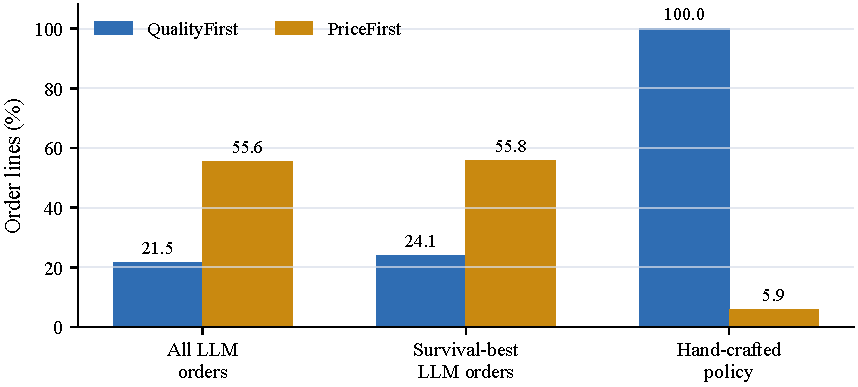
\includegraphics[width=\linewidth]{figures/supplier_selection_diagnostic.pdf}
\caption{Supplier-selection diagnostic used in Stage 3. \textbf{QualityFirst} is the fraction of order lines choosing the raw-quality-best supplier among candidates for the same product, while \textbf{PriceFirst} is the fraction choosing the cheapest supplier. The comparison shows that LLM orders are more price-first than quality-first, whereas the hand-crafted policy explicitly prioritizes supplier quality.}
\label{fig:supplier_selection_diagnostic}
\end{figure}

\paragraph{Stage 4: temporal follow-up.}
This stage measures whether the agent maintains stateful attention after actions and delayed consequences. Let $\mathcal{P}$ be the set of acted product-day pairs. For each $(j,t)\in\mathcal{P}$, let $b_{jt}=1$ if product $j$ receives another state-changing action within seven days, and otherwise $b_{jt}=0$. We also collect delayed event records $\mathcal{D}$, including stockout, return, and expiration events. Let $u_e=1$ if event $e\in\mathcal{D}$ receives no later query or action within the seven-day analysis window, and otherwise $u_e=0$. We report
\begin{equation}
\mathrm{FollowUp}
=\frac{1}{|\mathcal{P}|}\sum_{(j,t)\in\mathcal{P}} b_{jt},
\end{equation}
\begin{equation}
\mathrm{Resolved}
=1-\frac{1}{|\mathcal{D}|}\sum_{e\in\mathcal{D}}u_e.
\end{equation}
\textbf{FollowUp} captures whether products that received actions remain in the operational loop. \textbf{Resolved} captures whether delayed negative signals are later attended to through either a query or another state-changing action. Additional diagnostics track later query/action revisits, response latency in days, repeated events without intervention, and adjacent-day action-set continuity. Together, these metrics distinguish a one-shot daily policy from a policy that maintains product-level state across delayed feedback.
